%\documentclass[a4paper, 11pt]{article}
%\usepackage{amsmath}
%\usepackage{graphicx}
%\usepackage{geometry}
%\usepackage{listings}
%\usepackage{makecell}
%\usepackage{multirow}
%\geometry{scale=0.8}
%\linespread{1.5}
%\usepackage{hyperref}

\documentclass{article}
\usepackage[UTF8]{ctex}
\usepackage{listings}
\usepackage{xcolor}
\usepackage{enumerate}
\usepackage{array}
\usepackage{ulem}
\usepackage{amsmath}
\usepackage{makecell}
\usepackage{hyperref}
\usepackage{multirow}
\usepackage{titlesec} %自定义多级标题格式的宏包
\usepackage{graphicx, epsfig, psfrag}
\usepackage{subfigure}
\usepackage{geometry}
\geometry{a4paper,scale=0.8}
\linespread{1.5}

\title{	
\normalfont \normalsize
\textsc{School of Computer Science, Sun Yat-sen University} \\ [25pt] %textsc small capital letters
\rule{\textwidth}{0.5pt} \\[0.4cm] % Thin top horizontal rule
\huge  P02  CSP\\ % The assignment title
\rule{\textwidth}{2pt} \\[0.5cm] % Thick bottom horizontal rule
\author{Haoran Chen 19335016}
\date{\today}
}

\begin{document}
\maketitle
\tableofcontents
\newpage







\section{Futoshiki (GAC, C++/Python)}
\subsection{Description}
Futoshiki is a board-based puzzle game, also known under the name Unequal. It is playable on a square board having a given fixed size ($4\times4$ for example), please see Figure \ref{fig:futoshiki}.

The purpose of the game is to discover the digits hidden inside the board's cells; each cell is filled with a digit between 1 and the board's size. On each row and column each digit appears exactly once; therefore, when revealed, the digits of the board form a so-called Latin square.

At the beginning of the game some digits might be revealed. The board might also contain some inequalities between the board cells; these inequalities must be respected and can be used as clues in order to discover the remaining hidden digits.

Each puzzle is guaranteed to have a solution and only one.

You can play this game online: \url{http://www.futoshiki.org/}.
\begin{figure}[h]
  \centering
  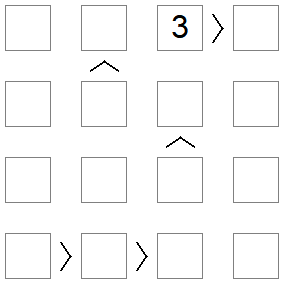
\includegraphics[width=6cm]{Pic/futoshiki1}
  \qquad
  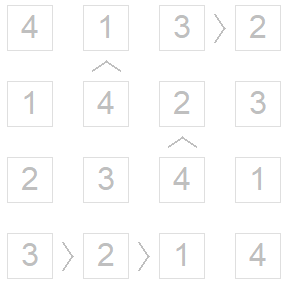
\includegraphics[width=6cm]{Pic/futoshiki2}
  \caption{Futoshiki Puzzles}
  \label{fig:futoshiki}
\end{figure}

\subsection{Tasks}

\begin{enumerate}
\item Describe with sentences the main ideas of the GAC algorithm and the main differences between the GAC and the forward checking (FC) algorithm. (10 points)\\
\textbf{Answer}: GAC算法的主要内容是检测每个变量的可扩展性以满足约束。即,如果变量的每个值都可以以满足约束的方式扩展到约束的其他变量,则变量与约束一致。至于他的优化问题, \\
GAC算法主要步骤如下:\\

\begin{figure}[!h]
    \centering
    \includegraphics[width=6in]{p1.bmp}   \caption{GAC算法主要步骤}
\end{figure}
\newpage
至于GAC与FC的区别,广义弧一致性(GAC, or弧相容, arc consistency)是前向检测的扩展, FC算法在运行过程中,每当一个新的变量被赋值,我们就能进行前向检测,并删去约束图中与刚赋值的变量相邻的未赋值变量的域;而GAC算法在运行过程中, 不仅仅是删去相邻的未赋值变量的域, 而是通过比较全部约束条件不断进行比较直到满足所有条件或者存储约束条件的队列变成空集, 效率较FC算法有较大提升.

\item The GAC$\_$Enforce procedure from class acts as follows: when removing d from CurDom[V], push all constraints $C'$ such that $V\in scope(C')$ and $C'\not\in$ GACQueue onto GACQueue. What's the reason behind this operation? Can it be improved and how? (20 points)\\
\textbf{Answer}:在进行操作removing d from CurDom[V]之后, CurDom[V]发生变化, 而与域V有关的约束$C'$受到操作影响也可能会导致与约束$C'$有关的其他变量域取值范围发生变化, 因此需要将与域V相关联且不在GACQueue的约束$C'$放入GACQueue中,这样能简化约束满足问题并且减少域的取值范围进而缩短搜索时间.这显然是可以优化的.\label{Node}一个简单的想法是,在GACQueue中取出一个约束条件后, 对其进行分类讨论, 如果是不等式约束, 将显然不符合不等关系的域中的值删除并标记是否删除,如果删除后域中没有值了,这显然是无解的;如果是行列关系,在判断在域范围大小是否为1后删除不符合约束条件的值并进行空域判断.

\item Use the GAC algorithm to implement a Futoshiki solver by \textbf{C++} or \textbf{Python}. (20 points)\\
    \textbf{Answer}: Please see the subsecion GAC Source Code in \ref{GAC Source Code}.

\item Explain any ideas you use to speed up the implementation. (10 points)\\
\textbf{Answer}: 见第二问\ref{Node}

\item Run the following 5 test cases to verify your solver's \textbf{correctness}. We also provide test file ``datai.txt" for every test case i. Refer to the ``readme.txt" for more details. (20 points)\\
\textbf{Answer}:运行结果如下:(图\ref{fig:case55}与\texttt{testcase5.txt}不一致)\\
\newpage
\begin{figure}[!h]
    \centering
    \subfigure[res1]{
        \includegraphics[width=2.4in]{res1.bmp}
        %\caption{res1}
    }
    \subfigure[res2]{
        \includegraphics[width=2.35in]{res2.bmp}
        %\caption{res2}
    }
    \subfigure[res3]{
        \includegraphics[width=2.3in]{res3.bmp}
        %\caption{res3}
    }
    \quad

\end{figure}

\begin{figure}[!h]
    \centering
    \subfigure[res4]{
        \includegraphics[width=2.12in]{res4.bmp}
        %\caption{res4}
    }
    \subfigure[res5]{
        \includegraphics[width=2in]{res5.bmp}
        %\caption{res5}
    }
    \caption{运行结果}
\end{figure}


\item Run the FC algorithm you implemented in E04 and the GAC algorithm you implemented in Task 3 on the 5 test cases, and fill in the following table. In the table,
    ``Total Time" means the total time the algorithm uses to solve the test case,  ``Number of Nodes Searched" means the total number of nodes traversed by the algorithm, 
    and ``Average Inference Time Per Node" means the average time for constraint propagation (inference) 
used in each node (note that this time is not equal to the total time divided by the number of nodes searched). Analyse the reasons behind the experimental results, and write them in your report. (20 points)\\
  
\setlength{\tabcolsep}{2mm}{

\begin{tabular}{|p{1.5cm}<{\centering}|p{2.2cm}<{\centering}|p{3cm}<{\centering}|p{3.3cm}<{\centering}|p{3.3cm}<{\centering}|}
\hline
Test Case&Algorithm&Total Time& Number of Nodes Searched&Average Inference Time Per Node\\
\hline
\multirow{2}*{1}& FC  &  0.002363 s  &    65    & 33.708 us/node \\
\cline{2-5}     & GAC &  0.001120 s  &    24    & 4.792 us/node \\
\hline
\multirow{2}*{2}& FC  &  0.002703 s  &    92    & 47.054 us/node \\
\cline{2-5}     & GAC &  0.001354 s  &    31    & 3.710 us/node \\
\hline
\multirow{2}*{3}& FC  &  0.052703 s  &   1328   & 69.760 us/node \\
\cline{2-5}     & GAC &  0.010813 s  &    80    & 121.600 us/node\\
\hline
\multirow{2}*{4}& FC  &  0.091053 s  &   1386   & 165.013 us/node \\
\cline{2-5}     & GAC &  0.055620 s  &    200   & 339.235 us/node \\
\hline
\multirow{2}*{5}& FC  &1702.582241 s & 26742542 & 81.598 us/node \\
\cline{2-5}     & GAC & 139.164101 s &  378766  & 407.133 us/node\\
\hline
\end{tabular}}
\\
  \\
  
可以看到, 不论在什么情况下, GAC算法搜索的节点数总是要小于FC算法搜索的节点数,在puzzle大小比较小且者约束条件比较多时, GAC算法与FC算法程序运行时间相差无几, 但是但问题规模比较大时, 性能差距就显现出来了(样例5的运行时间与搜索节点数差距十分明显); 至于每个节点的平均推断时间, 可以看到, 在问题规模小的时候, GAC的消耗时间是比FC小的, 甚至可以忽略不计, 但是但问题规模变大的时候, GAC的消耗时间逐渐增大, 超过了FC的平均推断时间.究其原因, 是因为GAC算法在实现弧一致性期间, 需要不断判断, 删除, 插入约束条件直到GacQueue为空, 在问题规模较大的时候, 这种不断地判断、插入与删除是比较消耗时间的,而且FC算法判断的条件相对来说比较少, 这就导致了在节点平均推断时间方面FC算法比较稳定, 而GAC在问题规模变大的情况下推断时间也随之变大.

    \begin{figure}[htbp]
    \centering
    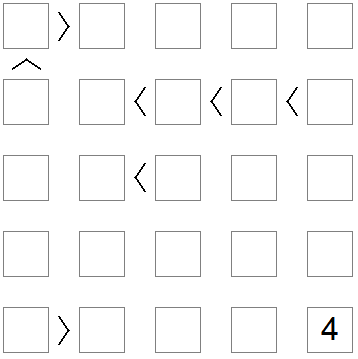
\includegraphics[width=5cm]{Pic/f1}
    \qquad
    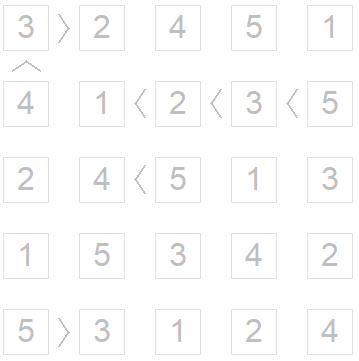
\includegraphics[width=5cm]{Pic/f1s}
    \caption{Futoshiki Test Case 1}
    \label{fig:case11}
  \end{figure}
        \begin{figure}[htbp]
    \centering
    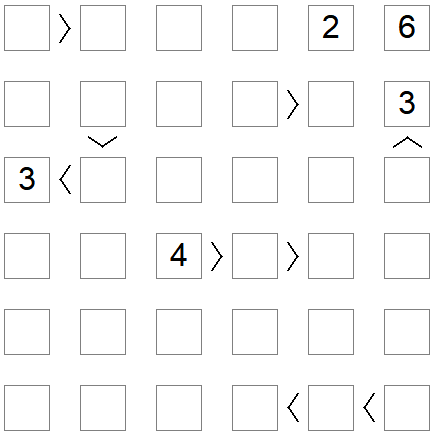
\includegraphics[width=5.5cm]{Pic/f2}
    \qquad
    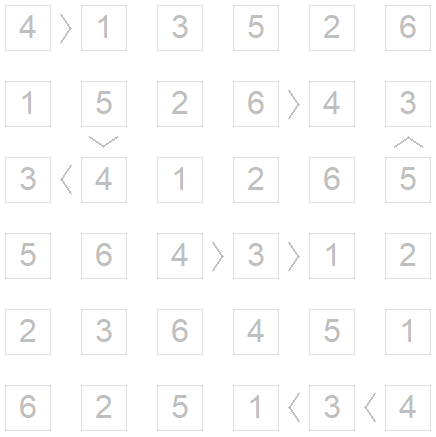
\includegraphics[width=5.5cm]{Pic/f2s}
    \caption{Futoshiki Test Case 2}
    \label{fig:case22}
  \end{figure}
        \begin{figure}[htbp]
    \centering
    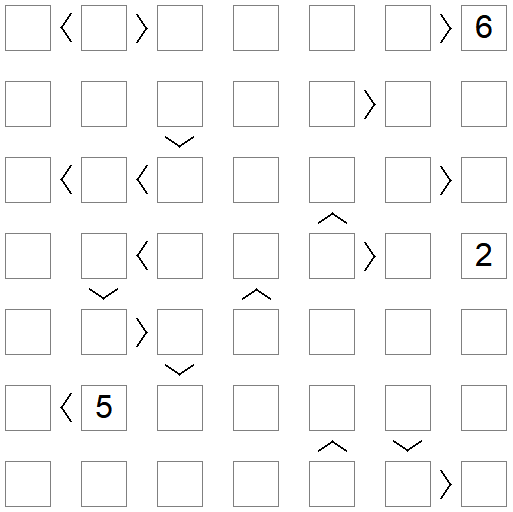
\includegraphics[width=6cm]{Pic/f3}
    \qquad
    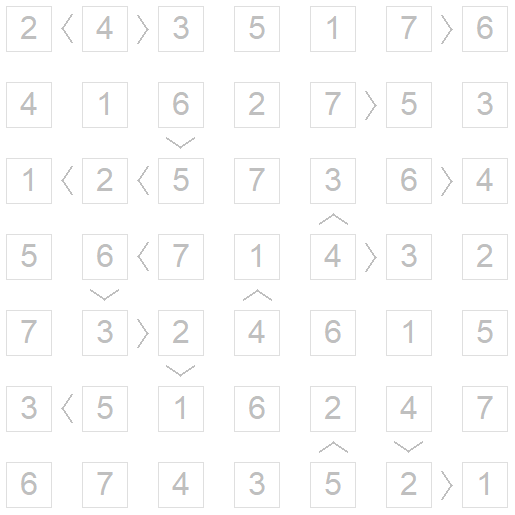
\includegraphics[width=6cm]{Pic/f3s}
    \caption{Futoshiki Test Case 3}
    \label{fig:case33}
  \end{figure}
        \begin{figure}[htbp]
    \centering
    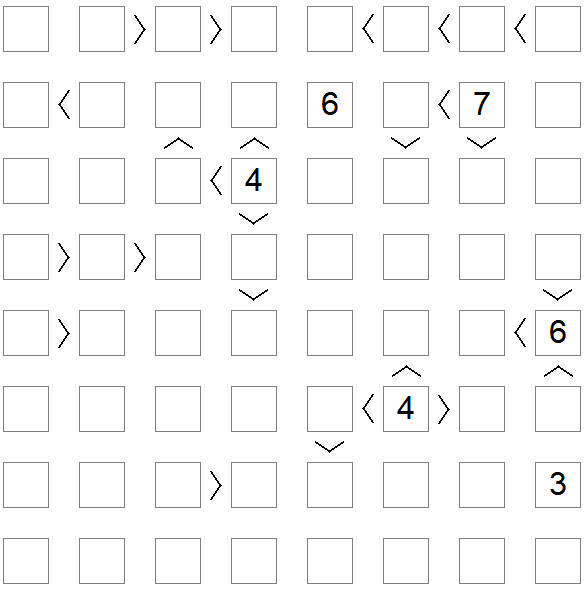
\includegraphics[width=6.5cm]{Pic/f4}
    \qquad
    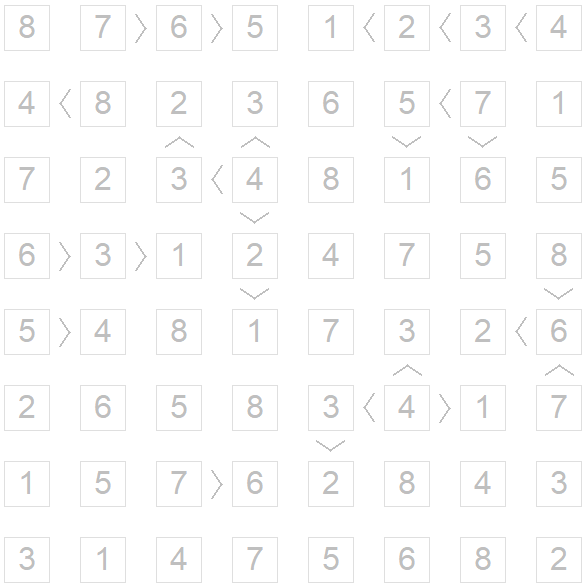
\includegraphics[width=6.5cm]{Pic/f4s}
    \caption{Futoshiki Test Case 4}
    \label{fig:case44}
  \end{figure}
        \begin{figure}[htbp]
    \centering
    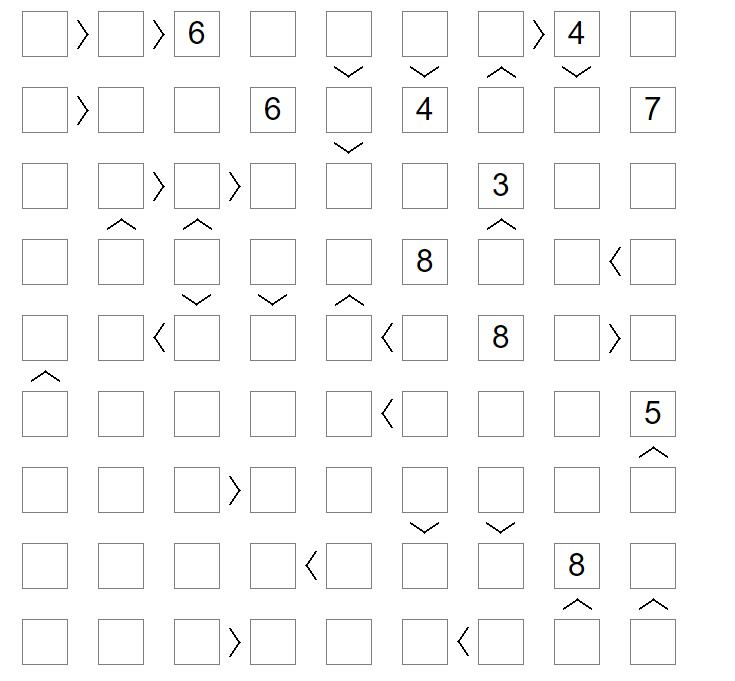
\includegraphics[width=7.5cm]{Pic/f5}
    \qquad
    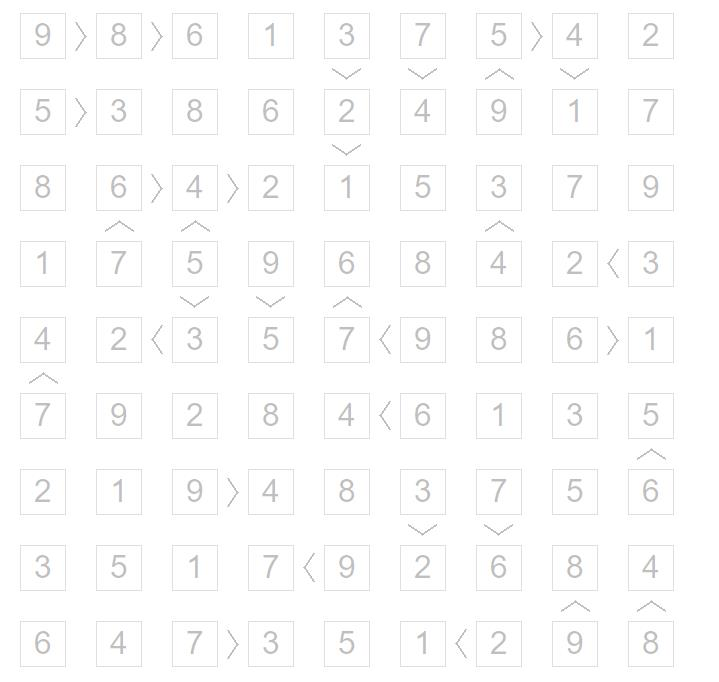
\includegraphics[width=7.5cm]{Pic/f5s}
    \caption{Futoshiki Test Case 5}
    \label{fig:case55}
  \end{figure}

\end{enumerate}

\section{To be announced}
\subsection{GAC Source Code}
\label{GAC Source Code}
\begin{lstlisting}[language = sql, numbers=left,numberstyle=\tiny,keywordstyle=\color{blue!70},commentstyle=\color{red!50!green!50!blue!50},frame=shadowbox,rulesepcolor=\color{red!20!green!20!blue!20},basicstyle=\ttfamily]
#include <iostream>
#include <fstream>
#include <sstream>
#include <vector>
#include <string>
#include <set>
#include <algorithm>
#include <list>
#include <ctime>
#include <windows.h>
using namespace std;

#define POINT pair<int, int>
#define PUZZLE vector<vector<int> >
#define DOMAINS vector<vector<set<int> > >

long long node_find = 0;

LARGE_INTEGER node_start_time, node_end_time, frequency;
long long count_time = 0;

struct Constraint {
    //0为不等式约束,>0为行约束,<0为列约束;
    //行列数从1开始计数, 且列值取负, 否则与不等式约束重复冲突。
    int type;
    // 不等式约束,relation.first < relation.second
    pair<POINT, POINT> relation;               
    Constraint(int t = 0, pair<POINT, POINT> r = {{-1, -1},{-1, -1}})
    : type(t), relation(r) {}
    //重载约束比较, 不加这个会报错
    bool operator==(const Constraint& rhs) { 
        return (type == rhs.type && relation == rhs.relation);
    }
};

class Solution{
    private:
    int size;     // puzzle尺寸, 通过读取文件确定
    PUZZLE puzzle;
    vector<Constraint> conArray; 
    public:
    Solution(const string filename){
        size = 0;
        ifstream fin(filename.c_str());
        string firstLine, tmp;
        int con_num = 0;
        //确定puzzle尺寸
        getline(fin, firstLine);
        stringstream ss;ss<<firstLine;
        while(ss>>tmp) size++;
        //重置文件指针
        fin.clear();fin.seekg(0);
        puzzle.assign(size, vector<int>(size, 0));
        
        for (int i = 0; i < size; i++)  for (int j = 0; j < size; j++) 
        fin >> puzzle[i][j];
        
        //确定约束条件个数
        while(getline(fin, firstLine)) con_num++;
        fin.clear();fin.seekg(0);
        for(int _=1; _<=size; _++) getline(fin, firstLine);
        
        for (int i = 0; i < con_num; i++) {
            int x1, y1, x2, y2;
            fin >> x1 >> y1 >> x2 >> y2;
            conArray.push_back(Constraint(0, {{x1, y1}, {x2, y2}}));
        }
        fin.close();
    }
    bool isSolved(){
        for (int i = 0; i < size; i++) for (int j = 0; j < size; j++) 
        if (puzzle[i][j] == 0)  return false;
        
        return true;
    }
    void printPuzzle(){
        for (int i = 0; i < size; i++) {
            for (int j = 0; j < size; j++) printf("%d ", puzzle[i][j]);
            puts("");
        }
        puts("=================");
    }
    void FilePrintPuzzle(const string filename){
        ofstream fout (filename.c_str());
        for (int i = 0; i < size; i++) {
            for (int j = 0; j < size; j++) fout<<puzzle[i][j]<<" ";
            fout<<'\n';
        }
        fout<<"=================\n";
        fout.close();
    }
    
    // 初始化每个棋盘格子域
    DOMAINS makeDomains(list<Constraint>& gacQ){
        // 初始化
        DOMAINS domains(size, vector<set<int>>(size, set<int>()));
        for (int i = 0; i < size; i++) for (int j = 0; j < size; j++){
            if (puzzle[i][j] == 0) for (int k = 1; k <= size; k++) 
            	domains[i][j].insert(k); 
            else domains[i][j].insert(puzzle[i][j]);
        }
        
        // 将所有行列约束加入gacQ
        for (int rc = 1; rc <= size; rc++) {
            gacQ.push_back(Constraint(rc));   
            gacQ.push_back(Constraint(-rc)); 
        }
        for (int i = 0; i < conArray.size(); i++) 
        gacQ.push_back(conArray[i]);
        
        return GacEnforce(domains, gacQ);  // 执行Gac_enforce
    }
    
    // MinimumPos, 与FC的MinimumPos不一样
    POINT MinimumPos(){
        for (int i = 0; i < size; i++) for (int j = 0; j < size; j++)
        	if (puzzle[i][j] == 0) return {i, j};
        
        return POINT();
    }
    
    // 在具体实现中, 队列使用C++ STL list
    // 把与变量pos相关的约束不重复地加入队列
    void AddConstraint2Q(POINT pos, list<Constraint>& gacQ){
        for (int i = 0; i < conArray.size(); i++) {
            if (conArray[i].type != 0) continue;// 不等式约束
            
            pair<POINT, POINT> relation = conArray[i].relation;
            if (pos == relation.first || pos == relation.second) {
                auto constr_position = find(gacQ.begin(), 
                gacQ.end(), conArray[i]);
                if (constr_position == gacQ.end())   // 不重复加入, 以下同理
                gacQ.push_back(conArray[i]);
            }
        }
        //行约束
        Constraint row_constraint(Constraint(pos.first + 1));
        auto row_position = find(gacQ.begin(), gacQ.end(), row_constraint);
        if (row_position == gacQ.end()) gacQ.push_back(row_constraint);  
        
        //列约束
        Constraint col_constraint(Constraint(-pos.second - 1));
        auto col_position = find(gacQ.begin(), gacQ.end(), col_constraint);
        if (col_position == gacQ.end()) gacQ.push_back(col_constraint);
    } 
    
    
    DOMAINS GacEnforce(DOMAINS domains, list<Constraint>& gacQ){
        while (!gacQ.empty()) {//类似于bfs
            Constraint constraint = gacQ.front(); gacQ.pop_front();
            // 已优化不等式约束
            if (constraint.type == 0) {
                POINT sp = constraint.relation.first;
                POINT lp = constraint.relation.second;
                int low = *domains[sp.first][sp.second].begin();
                for (int k = 1; k <= low; k++) {
                    bool flag = domains[lp.first][lp.second].erase(k);
                    if (flag) {//确定是否删除了, 好进行下一步操作, 以下同理
                        if (domains[lp.first][lp.second].size() == 0) 
                        return DOMAINS();  // DWO
                        AddConstraint2Q(lp, gacQ);
                    }
                }
                int high = *domains[lp.first][lp.second].rbegin();
                for (int k = high; k <= size; k++) {
                    bool flag = domains[sp.first][sp.second].erase(k);
                    if (flag) {
                        if (domains[sp.first][sp.second].size() == 0) 
                        	return DOMAINS();  // DWO
                        AddConstraint2Q(sp, gacQ);
                    }
                }
            }
            // 已优化行约束
            else if (constraint.type > 0) {
                int row = constraint.type - 1;
                //判断唯一取值是否符合要求, 以下同理
                for(int j = 0; j < size; j++) if(domains[row][j].size()==1){
                    int value = *domains[row][j].begin();
                    for (int jj = 0; jj < size; jj++) if (jj != j) {
                        bool flag = domains[row][jj].erase(value);
                        if (flag) {
                            if (domains[row][jj].size() == 0) 
                            	return DOMAINS();  // DWO
                            AddConstraint2Q({row, jj}, gacQ);
                        }
                    }
                }
            }
            // 已优化列约束
            else {
                int col = -constraint.type - 1;
                for(int i = 0; i < size; i++) if(domains[i][col].size()==1){
                    int value = *domains[i][col].begin();
                    for (int ii = 0; ii < size; ii++) if (ii != i) {
                        bool flag = domains[ii][col].erase(value);
                        if (flag) {
                            if (domains[ii][col].size() == 0) 
                            	return DOMAINS();  // DWO
                            AddConstraint2Q({ii, col}, gacQ);
                        }
                    }
                }
            }
        }
        return domains;
    }
    PUZZLE Gac(const DOMAINS& domains, list<Constraint>& gacQ){
        if (domains.size() == 0) return PUZZLE();   //DWO
        if (isSolved()) return puzzle;
        POINT pos = MinimumPos();
        set<int> field = domains[pos.first][pos.second];
        for (auto pd = field.begin(); pd != field.end(); pd++) {
            QueryPerformanceCounter(&node_start_time);
            
            puzzle[pos.first][pos.second] = *pd;
            // 在domains副本上修改,否则原iteration失效
            auto temp_domains = domains;          
            temp_domains[pos.first][pos.second].clear();
            temp_domains[pos.first][pos.second].insert(*pd);
            AddConstraint2Q(pos, gacQ);
            
            temp_domains = GacEnforce(temp_domains, gacQ);
            
            if (temp_domains.size() != 0) {  // not DWO
                node_find++;
                PUZZLE res = Gac(temp_domains, gacQ); //gac递归
                if (res.size() != 0) return res; 
            }
            QueryPerformanceCounter(&node_end_time);
            count_time+=(node_end_time.QuadPart-node_start_time.QuadPart)
            				*1000000 / frequency.QuadPart;
        }
        puzzle[pos.first][pos.second] = 0;  //重新置0
        return PUZZLE();                    // DWO
    }
};

int main() {
    QueryPerformanceFrequency(&frequency);
    for(int t = 1; t <= 5; t++){
        node_find = 0;
        LARGE_INTEGER start_time, end_time;
        
        string testcase = "TestCase/data"+to_string(t)+".txt";
        Solution game(testcase);
        list<Constraint> gacQ;
        game.printPuzzle();
        // 初始化各变量域并执行GacEnforce
        auto domains = game.makeDomains(gacQ); 
        
        QueryPerformanceCounter(&start_time);
        PUZZLE result = game.Gac(domains, gacQ);
        QueryPerformanceCounter(&end_time);
        
        long long dur_time = (end_time.QuadPart-start_time.QuadPart)*1000000 
                                / frequency.QuadPart;
        
        game.printPuzzle();
        string filename = "TestCase/res_gac"+to_string(t)+".txt";
        game.FilePrintPuzzle(filename);
        ofstream fout (filename.c_str());
        fout<<"Number of Nodes Searched is "<<node_find<<"\n";
        fout<<"Total Time is "<<dur_time<<" us\n\n";
        fout<<"Average Inference Time Per Node is ";
        fout<<1.0*count_time/node_find<<" us/node\n\n";
        fout.close();
        printf("Number of Nodes Searched is %lld\n", node_find);
        printf("Total Time is %lld us\n", dur_time);
        printf("Average Inference Time Per Node is %lf us/node\n\n"
                , 1.0*count_time/node_find);
    }
    puts("end");
    return 0;
}
\end{lstlisting}


%\clearpage
%\bibliography{E:/Papers/LiuLab}
%\bibliographystyle{apalike}
\end{document}
%%% Local Variables:
%%% mode: latex
%%% TeX-master: t
%%% End:
